% 13.  Logistic 增长曲线模型和Gompertz增长曲线模型是计量经济学等学科中的两个常用模型,可以用来拟合销售量的增长趋势。
%     记Logistic 增长曲线模型为 y_t = L / (1 + a exp(-kt)),记Gompertz增长曲线模型为 y_t = L exp(-b exp(-kt)),这两个模型中L的经济学意义都是销售量的上限。表13.33中给出的是某地区高压锅的销售量(单位:万台),为给出此两模型的拟合结果,请考虑如下的问题:
% 1)	Logistic 增长曲线模型是一个可线性化模型吗。如果给定 L=3000,是否是一个可线性化模型,如果是,试用线性化模型给出参数a和k的估计值。
% 2)	利用1)所得到的a和k的估计值和L=3000作为Logistic模型的拟合初值,对Logistic模型做非线性回归。
% 3)	取初值L(0)=3000, b(0)=30, k(0)=0.4,拟合Gompertz模型。并与Logistic 模型的结果进行比较。

\subsubsection{算法设计}

\paragraph{第(1)问} Logistic增长曲线模型如下,
\begin{equation}
    y_t = \frac{L}{1 + a e^{-kt}}
\end{equation}

当参数$L,a,k$均未知时,该模型不是一个可线性化模型。当给定$L=3000$时,则是一个可线性化模型,可转化为,
\begin{equation}
    \ln\left(\frac{L}{y_t} - 1\right) = \ln a - kt
\end{equation}

其中$a,k$为待估参数。上式左端为因变量,记为$y$,自变量为$t$,令$\beta_0 = \ln a$且$\beta_1 = -k$,则上式可表示为$y = \beta_0 + \beta_1 t$。在MATLAB中,可采用\texttt{regress}命令进行线性回归。

\paragraph{第(2)问} 利用第(1)问所得到的$a$和$k$的估计值和$L=3000$作为Logistic模型的拟合初值,对Logistic模型做非线性回归。在MATLAB中,可采用\texttt{nlinfit}命令进行非线性回归。

\paragraph{第(3)问} Gompertz模型定义如下,
\begin{equation}
    y_t = L e^{-b e^{-kt}}
\end{equation}

取初值$L_0=3000, b_0=30, k_0=0.4$,用\texttt{nlinfit}命令进行非线性回归分析。

\subsubsection{程序}

请参见附录\ref{sec:ex13_code}。

\subsubsection{计算结果}

\paragraph{第(1)问} 经过计算,得到回归模型参数如\Cref{tab:ex13_logistic_linear}。

\begin{table}[H]
    \centering
    \caption{Logistic回归模型}
    \label{tab:ex13_logistic_linear}
    \begin{tabular}{|c|c|c|}
        \hline
        回归系数 & 估计值 & 置信区间\\
        \hline
        \hline
        \(\beta_0\) & 3.8032 & [3.5765, 4.0299]\\
        \hline
        \(\beta_1\) & -0.4941 & [-0.5262, -0.4621]\\
        \hline
        \multicolumn{3}{|c|}{$R^2=0.9905, \quad F=1150.7545, \quad p=0.0000, \quad s^2=0.0386$}\\
        \hline
    \end{tabular}
\end{table}

计算参数$a,k$的估计值,
\begin{equation}
    \hat{a} = e^{\hat{\beta}_0} = 44.8463, \quad \hat{k} = -\hat{\beta}_1 = 0.4941
\end{equation}

画出拟合曲线,如\Cref{fig:ex13_logistic_linear},经过计算,其剩余标准差为$s=5053.0508$。

\begin{figure}[H]
    \centering
    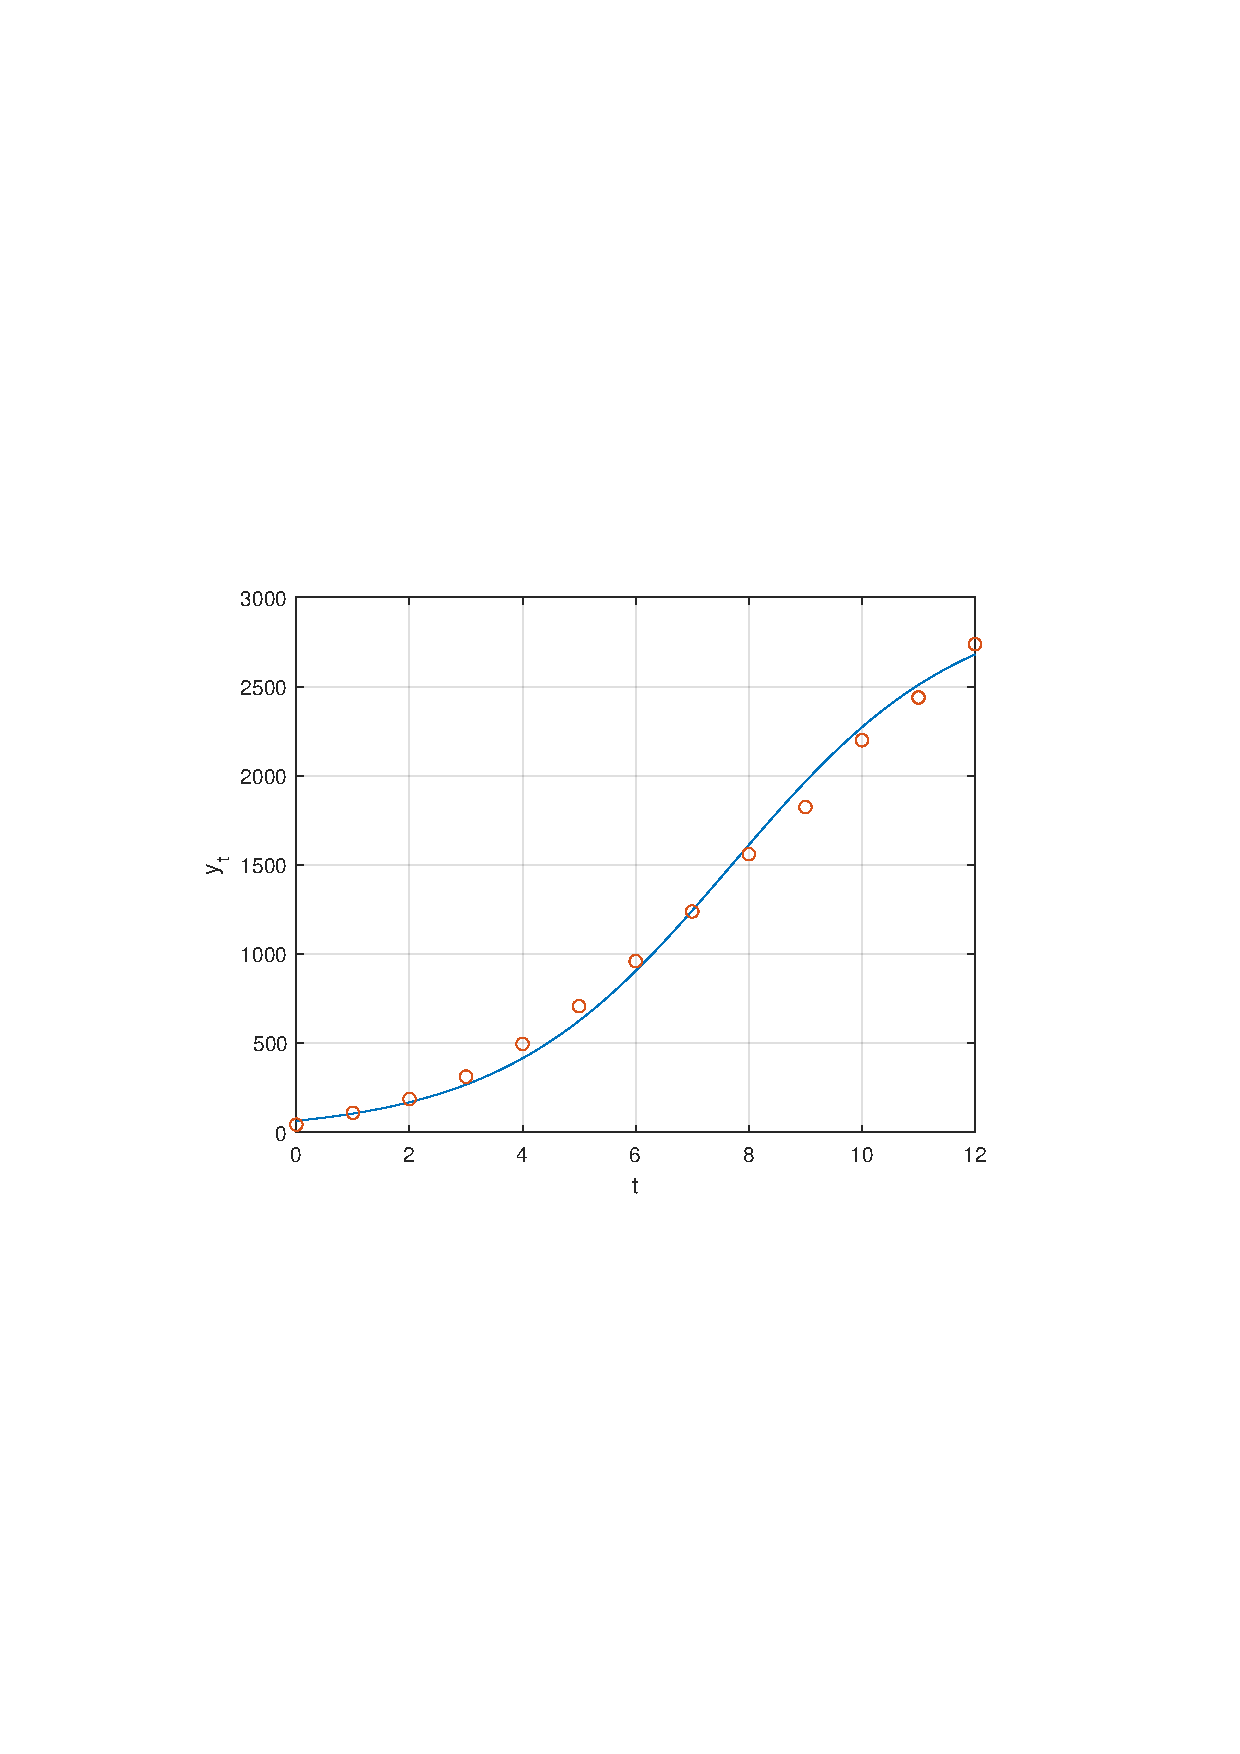
\includegraphics[width=0.8\textwidth,trim={3.09cm 9.295cm 3.09cm 9.295cm},clip]{fig/ex13_logistic_linear.pdf}
    \caption{Logistic线性回归模型拟合曲线}
    \label{fig:ex13_logistic_linear}
\end{figure}

\paragraph{第(2)问} 由第(1)问计算结果,可得非线性拟合的初值为$L_0 = 3000, a_0 = 44.8463, k_0 = 0.4941$,经过非线性回归,得到回归系数为,
\begin{equation}
    \hat{L} = 3260.4185, \quad \hat{a} = 30.5351, \quad \hat{k} = 0.4148
\end{equation}

画出拟合曲线,如\Cref{fig:ex13_logistic_nonlinear},其剩余标准差为$s=1765.1289$,模型的拟合效果比线性回归模型更好。

\begin{figure}[H]
    \centering
    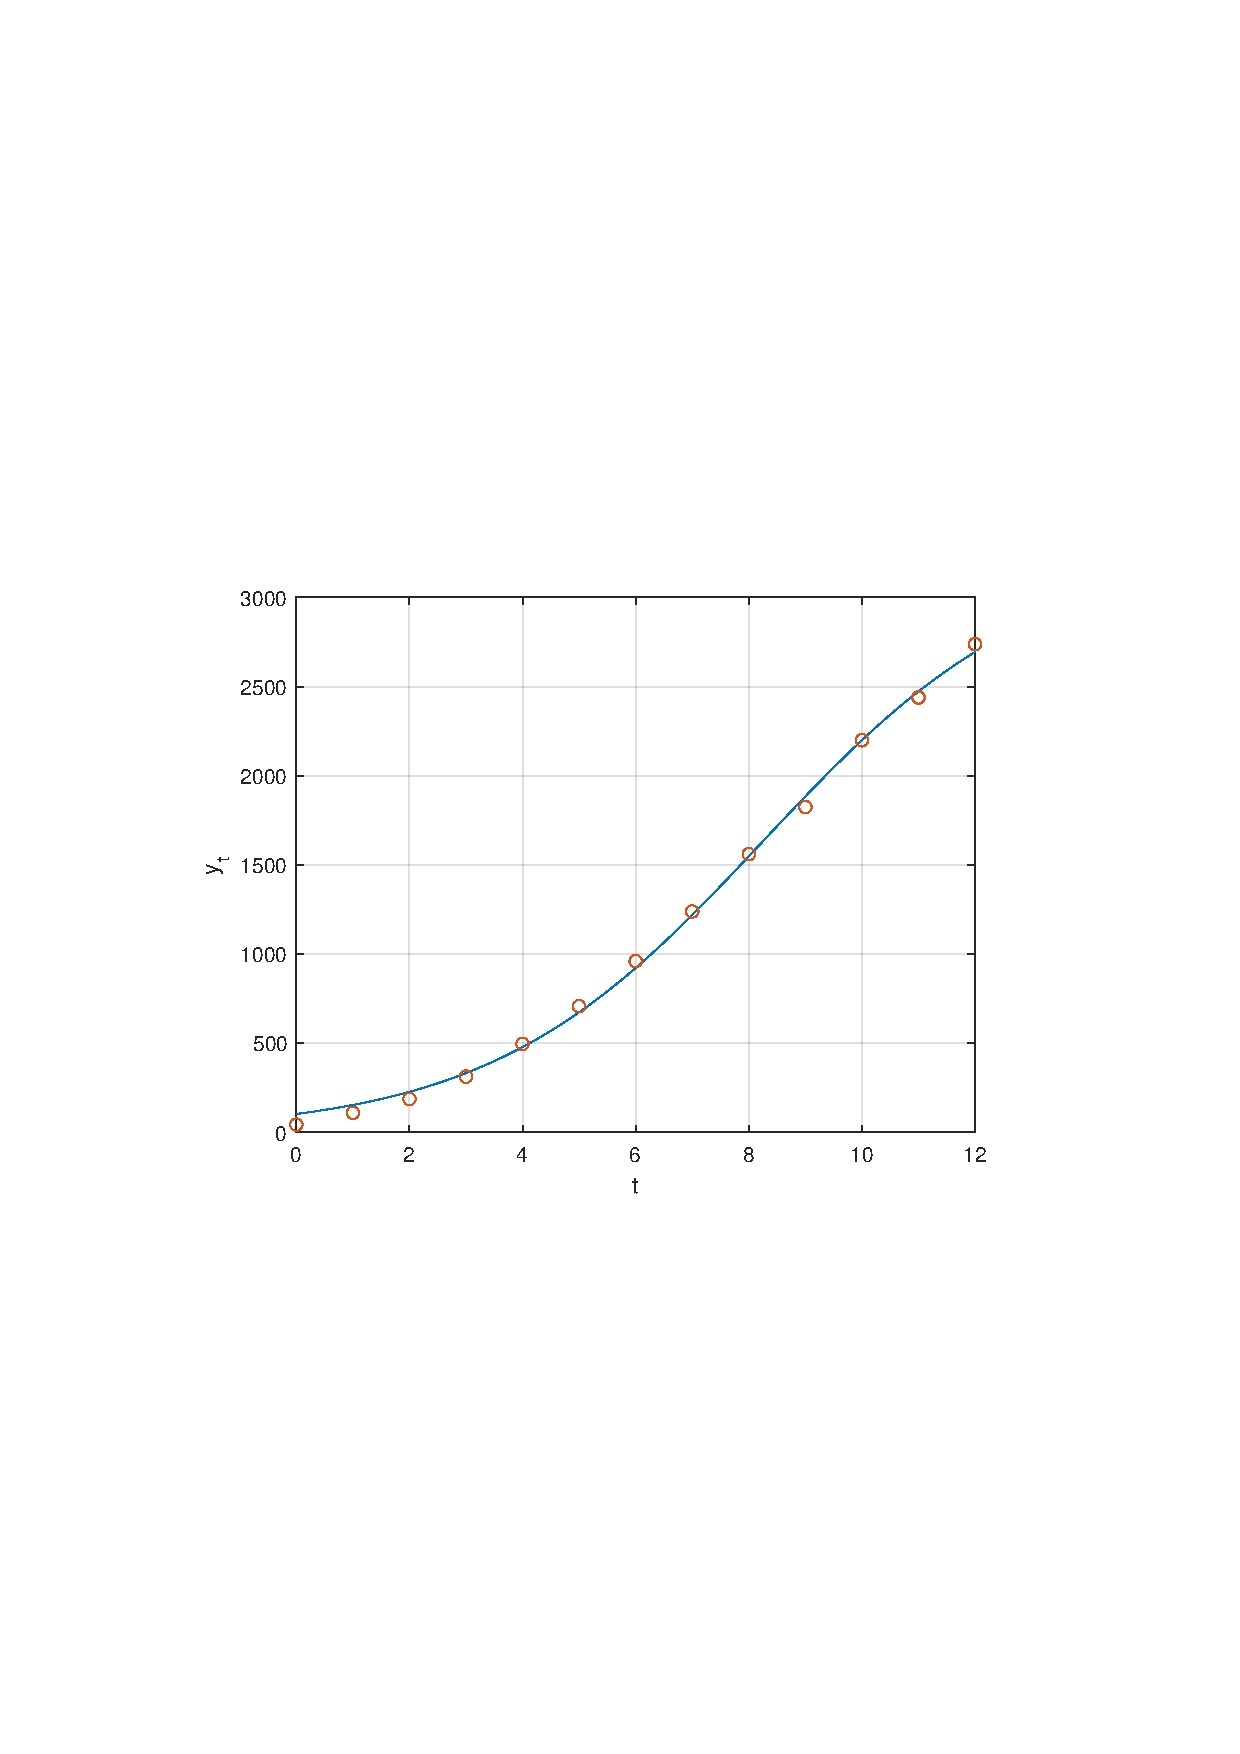
\includegraphics[width=0.8\textwidth,trim={3.09cm 9.295cm 3.09cm 9.295cm},clip]{fig/ex13_logistic_nonlinear.pdf}
    \caption{Logistic非线性回归模型拟合曲线}
    \label{fig:ex13_logistic_nonlinear}
\end{figure}

\paragraph{第(3)问} 以$L_0=3000, b_0=30, k_0=0.4$作为初值,经过非线性回归,得到Gompertz模型参数的估计值为,
\begin{equation}
    \hat{L} = 4810.1269, \quad \hat{b} = 4.5920, \quad \hat{k} = 0.1747
\end{equation}

画出拟合曲线,如\Cref{fig:ex13_gompertz_nonlinear},其剩余标准差为$s=308.1378$,低于Logistic模型,说明Gompertz模型比Logistic模型的拟合效果更好。

\begin{figure}[H]
    \centering
    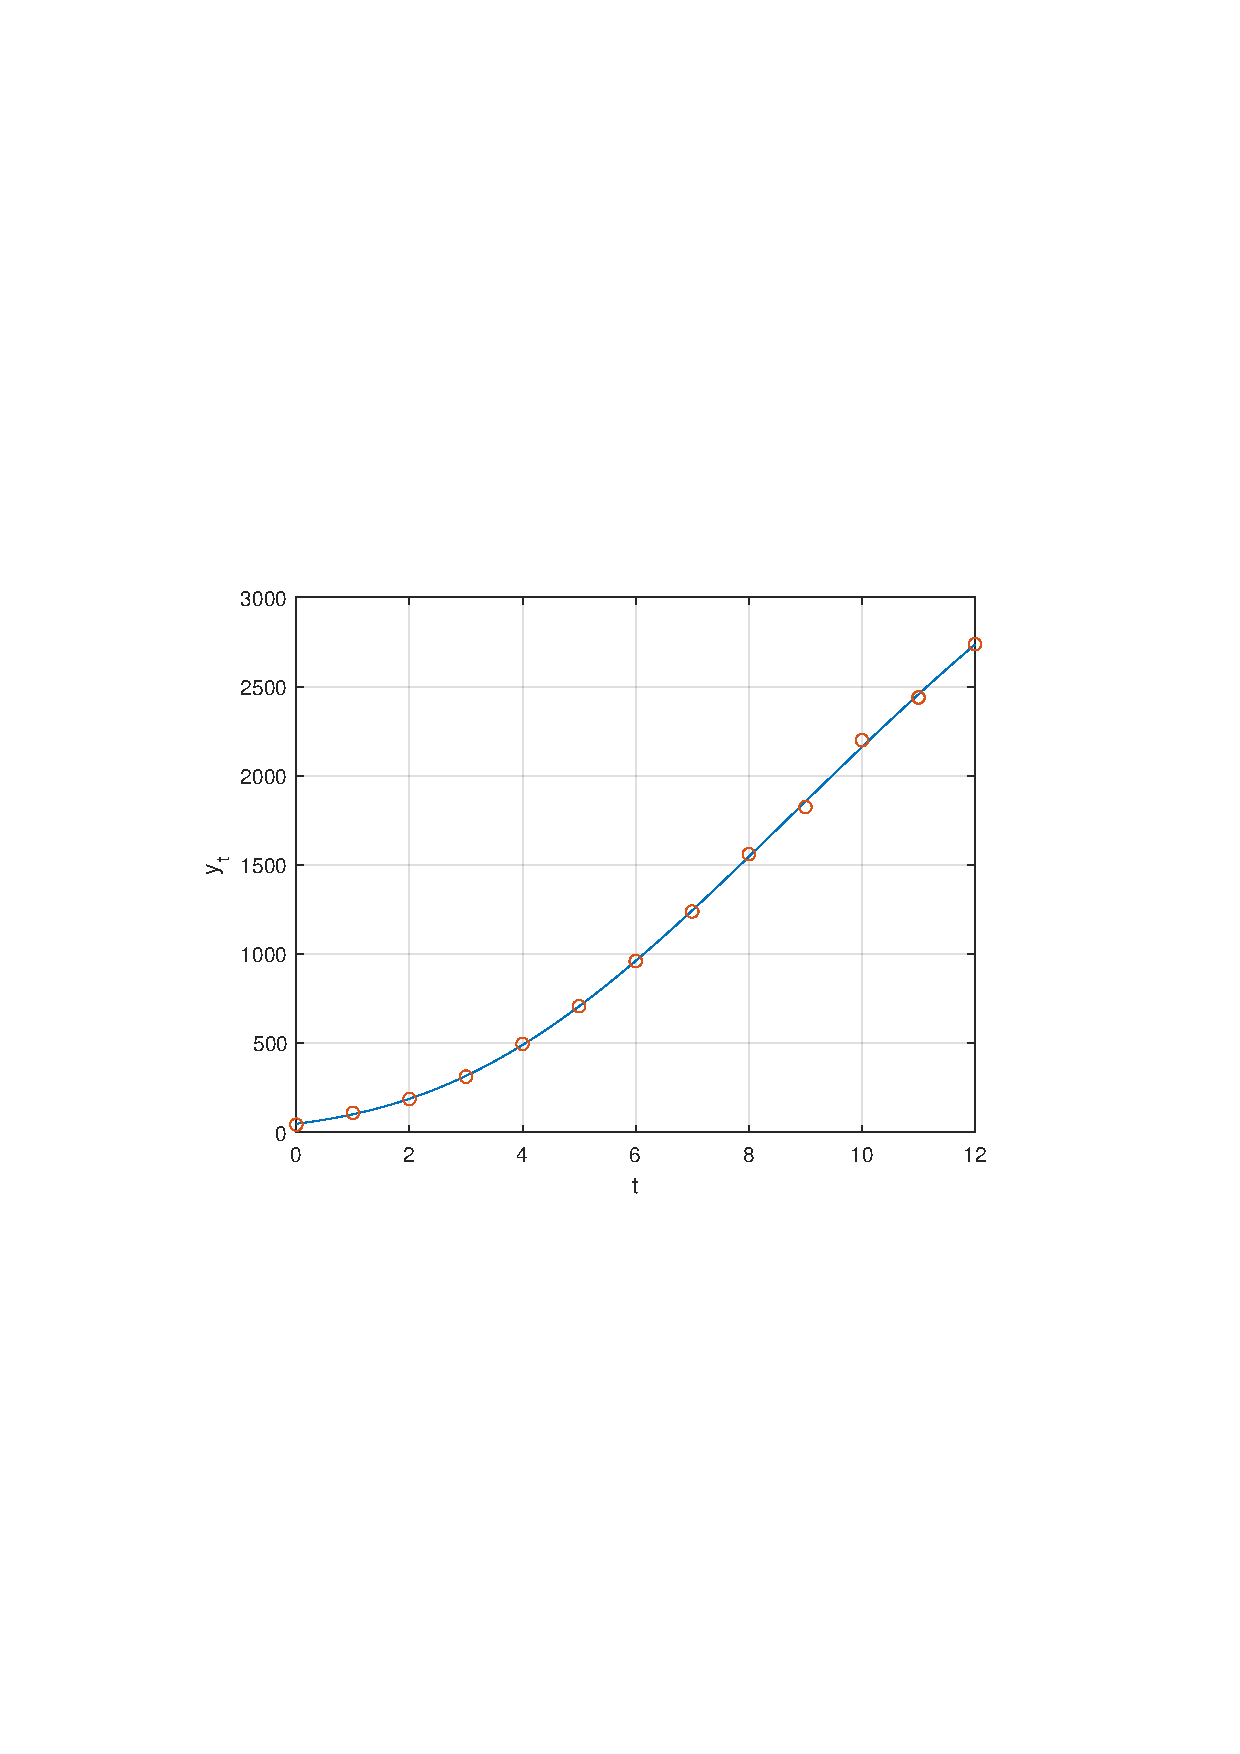
\includegraphics[width=0.8\textwidth,trim={3.09cm 9.295cm 3.09cm 9.295cm},clip]{fig/ex13_gompertz_nonlinear.pdf}
    \caption{Gompertz非线性回归模型拟合曲线}
    \label{fig:ex13_gompertz_nonlinear}
\end{figure}

\subsubsection{结果分析}

求解非线性回归模型时,选取合适的初值,可以降低计算量,加快收敛速度。如果模型可线性化,可以先求出线性化回归模型的参数估计值,将其作为初值,进一步求解非线性回归模型。

\subsubsection{结论}

Logistic增长曲线模型不是一个可线性化模型,如果给定$L=3000$,则是一个可线性化模型,用线性化模型给出参数$a$和$k$的估计值为$\hat{a} = 44.8463$和$\hat{k} = 0.4941$。

将上述$a$和$k$的估计值和$L=3000$作为Logistic模型的拟合初值,对Logistic模型做非线性回归,得到$\hat{L} = 3260.4185, \hat{a} = 30.5351, \hat{k} = 0.4148$。

取初值$L_0=3000, b_0=30, k_0=0.4$,拟合Gompertz模型,得到$\hat{L} = 4810.1269, \hat{b} = 4.5920, \hat{k} = 0.1747$,与Logistic模型相比,Gompertz模型的拟合效果更好。
